\documentclass[border=8pt]{standalone}
\usepackage[T1]{fontenc}\usepackage{helvet}\renewcommand{\familydefault}{\sfdefault}
\usepackage{tikz}\usetikzlibrary{positioning,arrows.meta,fit,backgrounds,calc,shadows.blur}
\definecolor{tudblue}{HTML}{0C2D48}\definecolor{tudcyan}{HTML}{00A6D6}
\definecolor{lgreen}{HTML}{D3EFDD}\definecolor{bgreen}{HTML}{27AE60}
\definecolor{lorange}{HTML}{FBE5CA}\definecolor{borange}{HTML}{F39C12}
\definecolor{dgray}{HTML}{E5E9ED}
\tikzset{
  base/.style={rectangle,rounded corners=3pt,draw=tudblue,very thick,align=center,
    inner sep=5pt,font=\footnotesize,minimum height=1.05cm,
    drop shadow={shadow xshift=1pt,shadow yshift=-1pt,opacity=0.18}},
  data/.style={base,fill=dgray,text width=3.7cm},
  gemini/.style={base,fill=tudcyan,text=white,text width=3.7cm},
  sft/.style={base,fill=tudcyan,text=white,text width=4.5cm},
  best/.style={base,fill=bgreen,text=white,text width=4.5cm,line width=1.1pt},
  grpo/.style={base,fill=tudblue,text=white,text width=4.7cm},
  eval/.style={base,fill=lgreen,draw=bgreen,text width=3.9cm},
  note/.style={base,fill=lorange,draw=borange,text width=4.7cm,font=\scriptsize},
  lab/.style={font=\bfseries\small,text=tudblue},
  ar/.style={-{Latex[length=2.4mm]},very thick,draw=tudblue},
}
\begin{document}
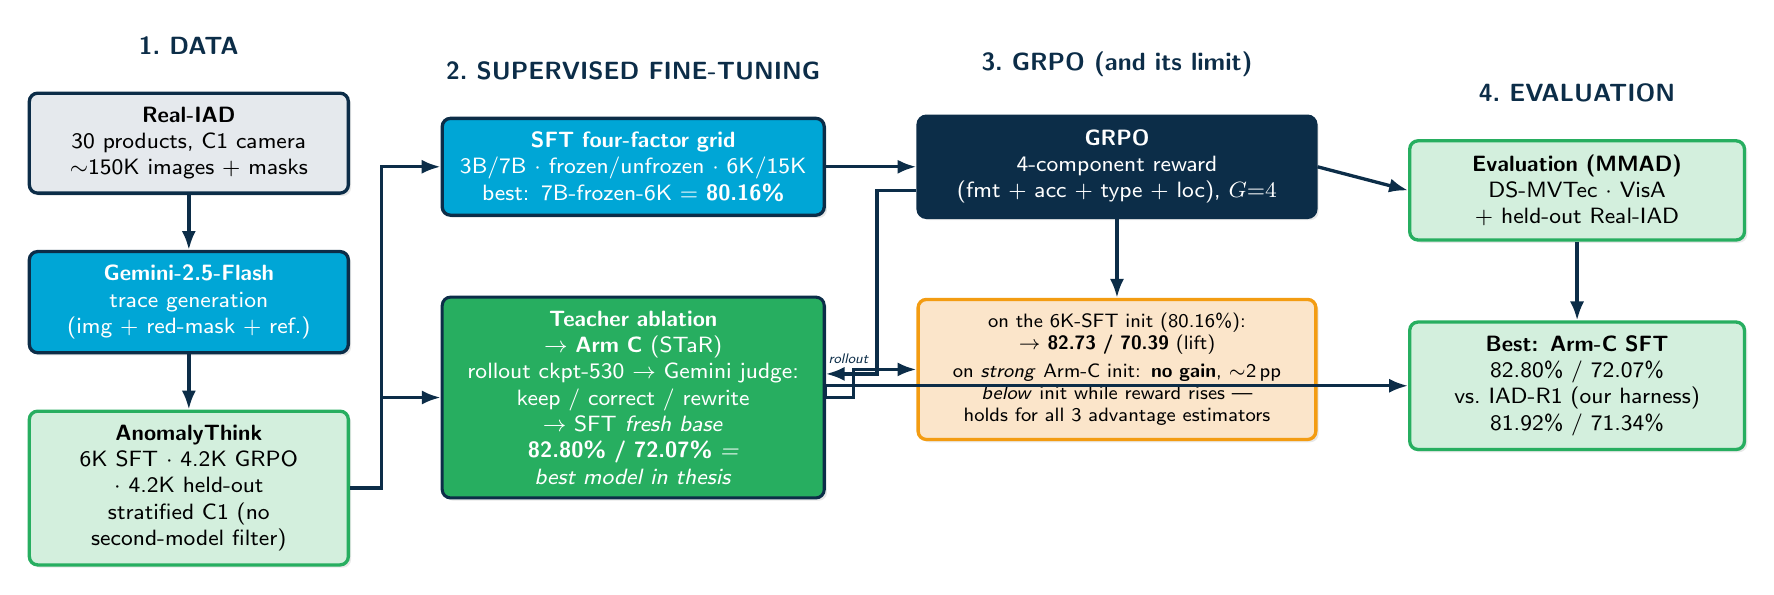
\begin{tikzpicture}[node distance=0.7cm and 1.15cm]
% ---- Stage 1: DATA ----
\node[data] (a1){\textbf{Real-IAD}\\30 products, C1 camera\\$\sim$150K images $+$ masks};
\node[gemini,below=of a1] (a2){\textbf{Gemini-2.5-Flash}\\trace generation\\(img $+$ red-mask $+$ ref.)};
\node[data,below=of a2,fill=lgreen,draw=bgreen] (a3){\textbf{AnomalyThink}\\6K SFT $\cdot$ 4.2K GRPO $\cdot$ 4.2K held-out\\stratified C1 (no second-model filter)};
\node[lab,above=0.35cm of a1]{1.\ DATA};
\draw[ar](a1)--(a2);\draw[ar](a2)--(a3);

% ---- Stage 2: SFT ----
\node[sft,right=of a1,yshift=-3mm] (b1){\textbf{SFT four-factor grid}\\3B/7B $\cdot$ frozen/unfrozen $\cdot$ 6K/15K\\best: 7B-frozen-6K $=$ \textbf{80.16\%}};
\node[best,below=1.0cm of b1] (b2){\textbf{Teacher ablation $\rightarrow$ Arm C} (STaR)\\rollout ckpt-530 $\rightarrow$ Gemini judge:\\keep / correct / rewrite $\rightarrow$ SFT \emph{fresh base}\\\textbf{82.80\% / 72.07\%} \textit{= best model in thesis}};
\node[lab,above=0.35cm of b1]{2.\ SUPERVISED FINE-TUNING};
\draw[ar](a3.east)-- ($(a3.east)+(0.4,0)$) |- (b1.west);
\draw[ar](a3.east)-- ($(a3.east)+(0.4,0)$) |- (b2.west);

% ---- Stage 3: GRPO ----
\node[grpo,right=of b1] (c1){\textbf{GRPO}\\4-component reward\\(fmt $+$ acc $+$ type $+$ loc), $G{=}4$};
\node[note,below=1.0cm of c1] (c2){on the 6K-SFT init (80.16\%): $\rightarrow$ \textbf{82.73 / 70.39} (lift)\\[2pt] on \emph{strong} Arm-C init: \textbf{no gain}, $\sim$2\,pp \emph{below} init while reward rises --- holds for all 3 advantage estimators};
\node[lab,above=0.35cm of c1]{3.\ GRPO (and its limit)};
\draw[ar](b1.east)--(c1.west);
\draw[ar](c1)--(c2);
\draw[ar]($(c1.west)+(0,-0.3)$) -- ++(-0.5,0) |- ($(b2.east)+(0,0.3)$)
  node[pos=0.78,above,font=\tiny\itshape,text=tudblue]{rollout};
\draw[ar](b2.east)-- ($(b2.east)+(0.35,0)$) |- (c2.west);

% ---- Stage 4: EVAL ----
\node[eval,right=of c1,yshift=-3mm] (d1){\textbf{Evaluation (MMAD)}\\DS-MVTec $\cdot$ VisA\\$+$ held-out Real-IAD};
\node[eval,below=1.0cm of d1,fill=lgreen] (d2){\textbf{Best: Arm-C SFT}\\82.80\% / 72.07\%\\\footnotesize vs.\ IAD-R1 (our harness)\\81.92\% / 71.34\%};
\node[lab,above=0.35cm of d1]{4.\ EVALUATION};
\draw[ar](b2.east)|- (d2.west);
\draw[ar](c1.east)--(d1.west);
\draw[ar](d1)--(d2);
\end{tikzpicture}
\end{document}
